%%%%%%%%%%%%%%%%%%%%%%%%%%%%%%%
%   Mathematische Ausdrücke   %
%%%%%%%%%%%%%%%%%%%%%%%%%%%%%%%

%%%Integrale
%Integral von 0 bis pi/2
\renewcommand{\intpihalbe}{\int_{0}^{\frac{\pi}{2}}}
\renewcommand{\intnullbisn}{\int_{0}^{n}}
\renewcommand{\inteinsbisn}{\int_{1}^{n}}

%%%Summen
\renewcommand{\summeeinsbisn}{\sum_{i = 1}^{n}}
\renewcommand{\summeeinsbisnpluseins}{\sum_{i = 1}^{n+1}}
\renewcommand{\summenullbisn}{\sum_{i = 0}^{n}}
\renewcommand{\summenullbisnpluseins}{\sum_{i = 0}^{n+1}}

%%%Produkte
\renewcommand{\produkteinsbisn}{\Pi_{i=1}^{n}}
\renewcommand{\produkteinsbisnpluseins}{\Pi_{i=1}^{n+1}}
\renewcommand{\produktnullbisn}{\Pi_{i=0}^{n}}
\renewcommand{\produktnullbisnpluseins}{\Pi_{i=0}^{n+1}}

%%%Limes
\renewcommand{\limesngegenunendlich}{\lim_{n \rightarrow \infty}}
\renewcommand{\limesngegenminusunendlich}{\lim_{n \rightarrow - \infty}}
\renewcommand{\limesxgegenunendlich}{\lim_{x \rightarrow \infty}}
\renewcommand{\limesxgegenminusunendlich}{\lim_{x \rightarrow - \infty}}

%%%%%%%%%%%%%%%%%%%%%%%%%%%%%%%%%%%%%%
%   Umrandungen um Matheausdruecke   %
%%%%%%%%%%%%%%%%%%%%%%%%%%%%%%%%%%%%%%

%Schwarzer Kasten um Ausdruck => Es muss $formel$ angegeben werden
\renewcommand*{\rectangled}[1]{\tikz[baseline=(char.base)]{
\node[shape=rectangle,draw,inner sep=2pt] (char){#1};}}
%Roter Kasten um Ausdruck => Es muss $formel$ angegeben werden
\renewcommand*{\redrectangled}[1]{\tikz[baseline=(char.base)]{
\node[shape=rectangle,draw,inner sep=2pt, red] (char) {\textcolor{black}{#1}};}}
%Schwarzer Kreis um Ausdruck => Es muss $formel$ angegeben werden
\renewcommand*\circled[1]{\tikz[baseline=(char.base)]{
\node[shape=circle,draw,inner sep=1pt] (char) {#1};}}
%Roter Kreis um Ausdruck => Es muss $formel$ angegeben werden
\renewcommand*\redcircled[1]{\tikz[baseline=(char.base)]{
\node[shape=circle,draw,inner sep=1pt] (char) {\textcolor{red}{#1}};}}

%%%%%%%%%%%%%%%%%%%%%%%%%%%%%%%%%%%%%%%%%%%%%%%%%%%%%%%%%%%
%%%%%%%%%%%%%%%%%%%%%%%%%%%%%%%
%   Neue nützliche Commands   %
%%%%%%%%%%%%%%%%%%%%%%%%%%%%%%%

%%%%%%%%%%%%%%%%%%%%%%%%%%%%%%%%%%%%%%%%%%%%%%%%%%%%%%%%%%%

\subsection{Heapsort}


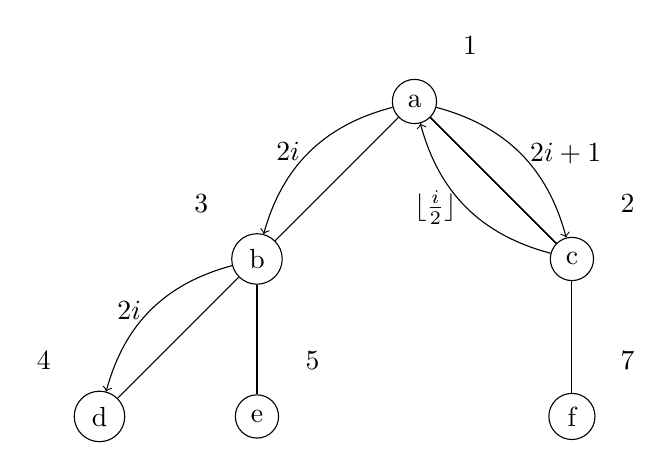
\begin{tikzpicture}[state/.style={draw, circle}]
\node(1) at (0,0) [state]{a };
\node(2) at (2,-2) [state]{c };
\node(3) at (-2,-2) [state]{b };
\node(4) at (-4,-4) [state]{d };
\node(5) at (-2,-4) [state]{e };
\node(7) at (2,-4) [state]{f };
\node(11)  [ above right  of= 1]{1 };
\node(21)  [ above right  of= 2]{2 };
\node(31)  [ above left  of= 3]{3 };
\node(41)  [ above left  of= 4]{4 };
\node(51)  [ above right  of= 5]{5 };
\node(71)  [ above right  of= 7]{7 };
\draw[-] (1) to (2);
\draw[-] (1) to (3);
\draw[-] (1) to (2);
\draw[-] (3) to (4);
\draw[-] (3) to (5);
\draw[-] (2) to (7);
\draw[-] (1) to (2);
\draw[-] (1) to (2);
\draw[->] (1) [bend right]to node[left]{$2i$} (3);
\draw[->] (1) [bend left]to node[right]{$2i+1$} (2);
\draw[->] (3) [bend right]to node[left]{$2i$} (4);
\draw[->] (2) [bend left] to node [left]{$\lfloor\frac{i}{2}\rfloor$} (1);
\end{tikzpicture}\\

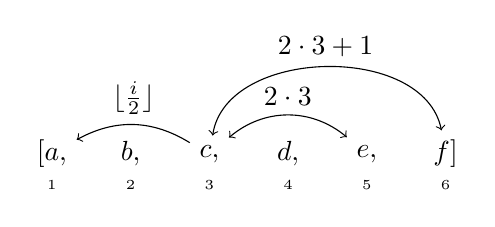
\begin{tikzpicture}
\node(1) at (0,0) [] {$[a,$};
\node(2) at (1,0) [] {$b,$};
\node(3) at (2,0) [] {$c,$};
\node(4) at (3,0) [] {$d,$};
\node(5) at (4,0) [] {$e,$};
\node(6) at (5,0) [] {$ f]$};
\node(11) at (0,-0.4) [] {\tiny $1$};
\node(21) at (1,-0.4) [] {\tiny $2$};
\node(31) at (2,-0.4) [] {\tiny $3$};
\node(41) at (3,-0.4) [] {\tiny $4$};
\node(51) at (4,-0.4) [] {\tiny $5$};
\node(61) at (5,-0.4) [] {\tiny $6$};
\draw[->] (3) [bend right]to node[above] {$\lfloor\frac{i}{2}\rfloor$} (1);
\draw[<->] (3) [bend left=4em]to node[above]{$2 \cdot 3$} (5);
\draw[<->] (3) [bend left=8em]to node[above]{$2 \cdot 3 + 1$} (6);
\end{tikzpicture}

\begin{align*}
    \log_2 (n) = \frac{\log_e(n)}{\log_e(2)}
\end{align*}


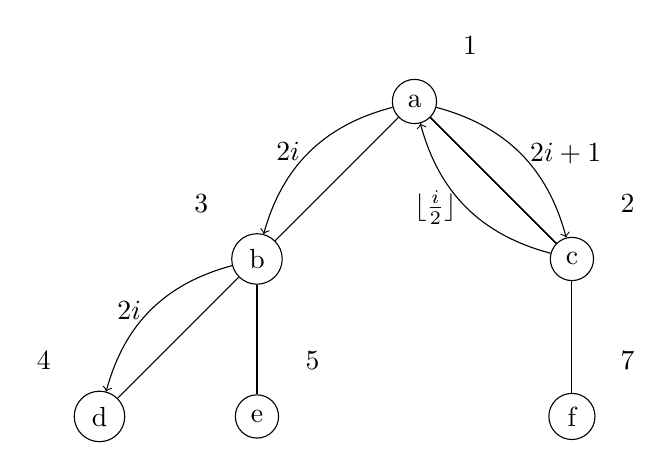
\begin{tikzpicture}[state/.style={draw, circle}]
\node(1) at (0,0) [state]{a };
\node(2) at (2,-2) [state]{c };
\node(3) at (-2,-2) [state]{b };
\node(4) at (-4,-4) [state]{d };
\node(5) at (-2,-4) [state]{e };
\node(7) at (2,-4) [state]{f };
\node(11)  [ above right  of= 1]{1 };
\node(21)  [ above right  of= 2]{2 };
\node(31)  [ above left  of= 3]{3 };
\node(41)  [ above left  of= 4]{4 };
\node(51)  [ above right  of= 5]{5 };
\node(71)  [ above right  of= 7]{7 };
\draw[-] (1) to (2);
\draw[-] (1) to (3);
\draw[-] (1) to (2);
\draw[-] (3) to (4);
\draw[-] (3) to (5);
\draw[-] (2) to (7);
\draw[-] (1) to (2);
\draw[-] (1) to (2);
\draw[->] (1) [bend right]to node[left]{$2i$} (3);
\draw[->] (1) [bend left]to node[right]{$2i+1$} (2);
\draw[->] (3) [bend right]to node[left]{$2i$} (4);
\draw[->] (2) [bend left] to node [left]{$\lfloor\frac{i}{2}\rfloor$} (1);
\end{tikzpicture}\\

\begin{align*}
    \sum_{h = 0}^{\lfloor \log n \rfloor} \frac{n}{2^{h+1}} \cdot O(h) = O(n \cdot \underbrace{\sum_{h = 0}^{\lfloor \log n \rfloor} \frac{h}{2^{h+1}}}_{c}) = O(n)
\end{align*}



\subsection{Weiteres}
Es gibt an dieser Stelle keine weiteren Mitschriften zu dieser Vorlesung, da die Tafelanschriften nicht hilfreich sind zum nachlesen.\\

Unter dem folgenden Link ist der Heapsort Algorithmus nocheinmal erklärt, wie in den Vorlesungen, sowohl in der Baumdarstellung, als auch in der Array-Darstellung.\\
\href{https://de.wikiversity.org/wiki/Kurs:Algorithmen_und_Datenstrukturen/Vorlesung/Heap_Sort_Vorgehensweise}{\nolinkurl{wikiversity}}
\\
Oder auch in den Folien von DAP2 aus dem Jahr 2019, ist der Algorithmus deutlich erklärt:(Wenn man in den Kurs eingeschrieben ist)\\
\href{https://moodle.tu-dortmund.de/pluginfile.php/895824/mod_resource/content/0/Vorlesung13-Datenstrukturen-III.pdf}{\nolinkurl{moodle-tudortmund}}
